% Koko
\documentclass[blue,normal,cn]{elegantnote}
\usepackage{array}
\usepackage{courier}
\usepackage{xcolor}
\usepackage{tabulary}
\usepackage{float}
\usepackage{makecell}
\usepackage{multirow}
\usepackage{zhnumber}

\definecolor{light-gray}{gray}{0.95}
\newcommand{\code}[1]{\colorbox{light-gray}{\texttt{#1}}}
\newfontfamily\courier{Courier New}
\lstset{linewidth=1.1\textwidth,
	numbers=left,
	basicstyle=\small\courier,
	numberstyle=\tiny\courier,
	keywordstyle=\color{blue}\courier,
	commentstyle=\it\color[cmyk]{1,0,1,0}\courier, 
	stringstyle=\it\color[RGB]{128,0,0}\courier,
	frame=single,
	backgroundcolor=\color[RGB]{245,245,244},
	breaklines,
	extendedchars=false, 
	xleftmargin=2em,xrightmargin=2em, aboveskip=1em,
	tabsize=4, 
	showspaces=false
	basicstyle=\small\courier
}
\title{分布式温控系统用例模型}
\version{1.0.0}
\date{\zhtoday}

\begin{document}
\author{
    \begin{tabular}[t]{c}
        2017211305 班 E 组 \\
        于海鑫\ 徐翔\ 赵泉斌\ 郭朝宇\ 郭璐
    \end{tabular}
}
\maketitle

\section{文档介绍}

\subsection{文档目的}
该文档主要目的在于建立用例模型。即根据已经确定的需求分析来描述用户以及各个子功能系统之间的交互场景。 对于每一个场景建立相应的用例模型, 软件开发人员应当根据此模型来进行软件的详细设计与开发。

\subsection{文档范围}
该文档围绕分布式温控系统展开,详细地描述分布式温控系统的用例图、用例说明以及操作契约等。 通过用例图构建出所有可能用例与各个参与者之间的框架结构关系, 然后对每一个交互场景进行详细描述和分析。

\subsection{读者对象}

\begin{itemize}
    \item 用户
    \item 设计人员
    \item 编码人员和测试人员等
\end{itemize}

\subsection{参考文献}

\begin{itemize}
    \item 《\emph{软件工程模型与方法}》 肖丁等\ 北京邮电大学出版社
    \item 《\emph{用户需求说明书}》\ 2017211305 班 E 组
\end{itemize}

\subsection{人员分工}

\begin{center}
    \begin{tabular}{cc}
        \toprule
        \textbf{组员} & \textbf{分工}        \\
        \midrule
        于海鑫        & 整合用例模型         \\
        郭朝宇        & 负责入住客户用例模型 \\
        赵泉斌        & 负责前台人员用例模型 \\
        郭璐          & 负责维护人员用例模型 \\
        徐翔          & 负责财务人员用例模型 \\
        \bottomrule
    \end{tabular}
\end{center}

\section{角色定义}

\begin{center}
    \begin{tabular}{cc}
        \toprule
        \textbf{角色名称} & \textbf{角色职责}                                \\
        \midrule
        入住客户          & 入住酒店,自助调节空调温度,支付空调费用         \\
        前台人员          & 协助客户办理入住、退房手续                       \\
        维护人员          & 监视并控制各房间空调状态,查看各房间空调使用情况 \\
        财务人员          & 查看温控报表                                     \\
        \bottomrule
    \end{tabular}
\end{center}

\section{用例定义}

\subsection{注册账号}
\subsubsection{用例图}

\begin{figure}[H]
    \centering
    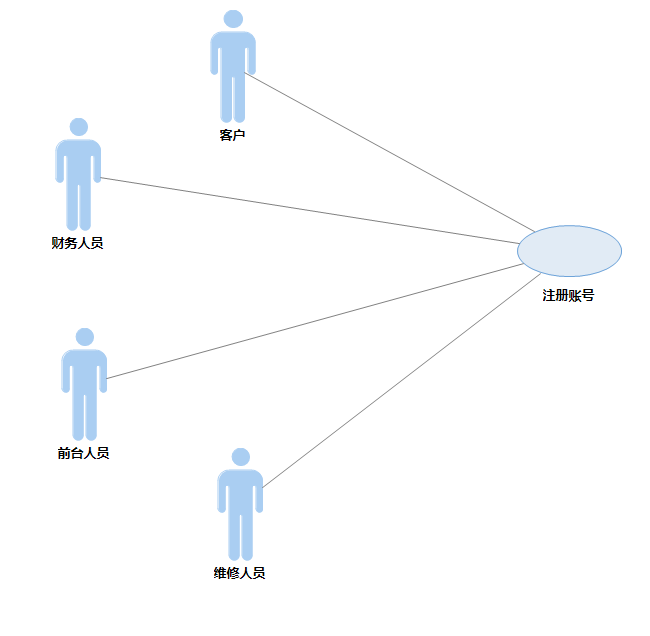
\includegraphics[width=.5\textwidth]{fig/276005.png}
    \caption{用例图:注册账号}
    \label{fig:276005}
\end{figure}

\subsubsection{系统顺序图}

\begin{figure}[H]
    \centering
    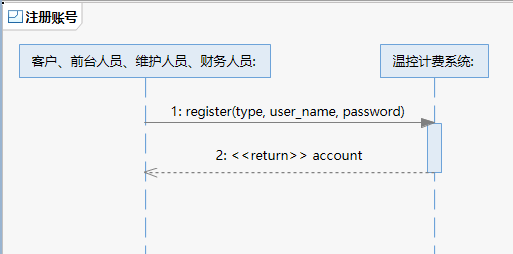
\includegraphics[width=.8\textwidth]{fig/276006.png}
    \caption{系统顺序图:注册账号}
    \label{fig:276006}
\end{figure}

\subsubsection{操作契约}

\begin{center}
    \begin{tabular}{|>{\centering}m{0.15\textwidth}|m{0.7\textwidth}|}
        \hline
        系统事件                  & \multicolumn{1}{l|}{\code{register(type, user\_name, password)}} \\
        \hline
        交叉引用                  & 注册账号                                                         \\
        \hline
        前置条件                  & 操作者想要在系统上注册账号                                       \\
        \hline
        \multirow{4}{*}{后置条件} & 一个新的(概念类)账号被创建                                     \\
        \cline{2-2}
                                  & 账号与操作者(客户、前台人员、维护人员、财务人员)建立关联       \\
        \cline{2-2}
                                  & 账号与温控计费系统建立关联                                       \\
        \cline{2-2}
                                  & 账号的属性初始化:类型,用户名,密码等                           \\
        \hline
    \end{tabular}
\end{center}

\subsection{登入系统}
\subsubsection{用例图}

\begin{figure}[H]
    \centering
    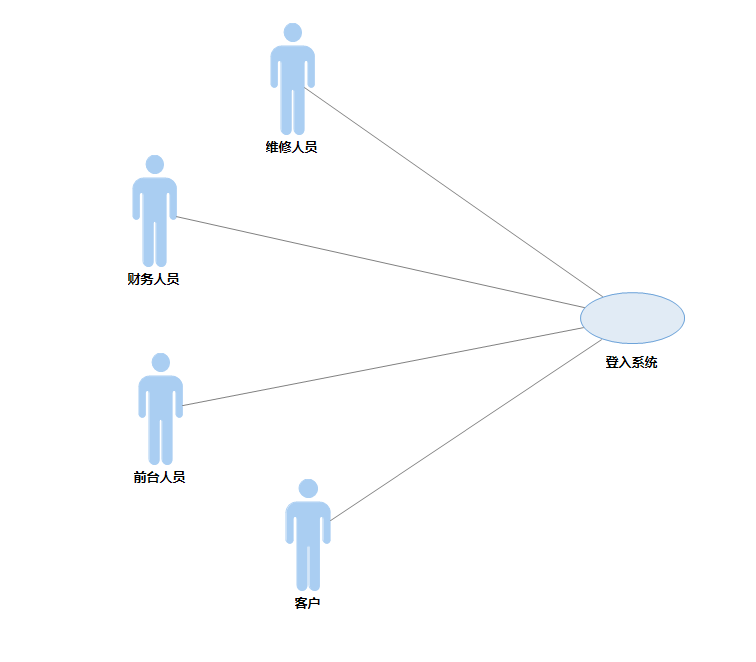
\includegraphics[width=.5\textwidth]{fig/276007.png}
    \caption{用例图:登入系统}
    \label{fig:276007}
\end{figure}

\subsubsection{系统顺序图}

\begin{figure}[H]
    \centering
    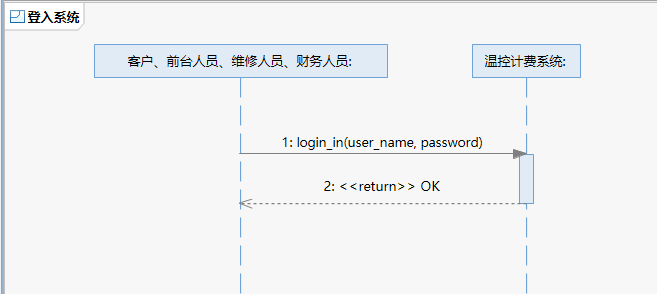
\includegraphics[width=.8\textwidth]{fig/276008.png}
    \caption{系统顺序图:登入系统}
    \label{fig:276008}
\end{figure}

\subsubsection{操作契约}

\begin{center}
    \begin{tabular}{|>{\centering}m{0.15\textwidth}|m{0.7\textwidth}|}
        \hline
        系统事件                  & \multicolumn{1}{l|}{\code{login\_in(user\_name, password)}} \\
        \hline
        交叉引用                  & 登入系统                                                    \\
        \hline
        前置条件                  & 操作者想要登入温控计费系统                                  \\
        \hline
        \multirow{1}{*}{后置条件} & 用户被赋予相应权限                                          \\
        \hline
    \end{tabular}
\end{center}

\subsection{登出系统}
\subsubsection{用例图}

\begin{figure}[H]
    \centering
    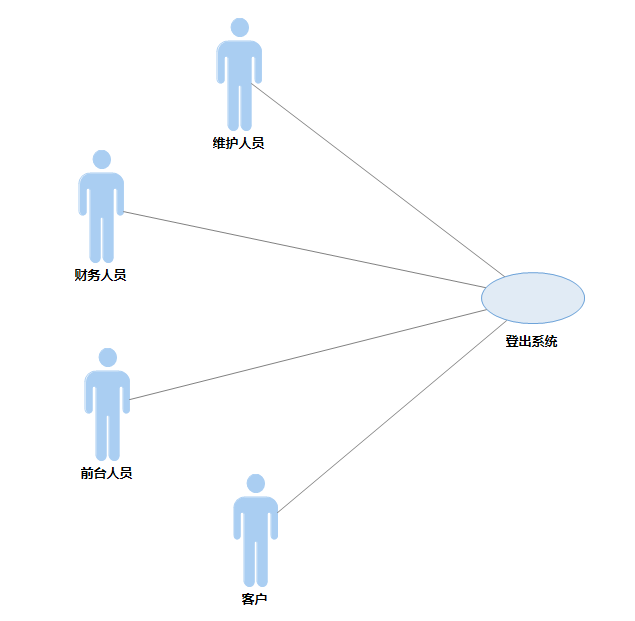
\includegraphics[width=.5\textwidth]{fig/276009.png}
    \caption{用例图:登出系统}
    \label{fig:276009}
\end{figure}

\subsubsection{系统顺序图}

\begin{figure}[H]
    \centering
    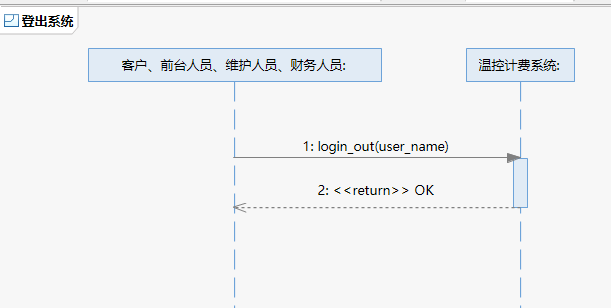
\includegraphics[width=.8\textwidth]{fig/276010.png}
    \caption{系统顺序图:登出系统}
    \label{fig:276010}
\end{figure}

\subsubsection{操作契约}

\begin{center}
    \begin{tabular}{|>{\centering}m{0.15\textwidth}|m{0.7\textwidth}|}
        \hline
        系统事件                  & \multicolumn{1}{l|}{\code{login\_out(user\_name)}} \\
        \hline
        交叉引用                  & 登出系统                                           \\
        \hline
        前置条件                  & 操作者想要登出温控计费系统                         \\
        \hline
        \multirow{1}{*}{后置条件} & 登出的IP被删除相应权限                             \\
        \hline
    \end{tabular}
\end{center}

\subsection{查看统计报表}
\subsubsection{用例图}

\begin{figure}[H]
    \centering
    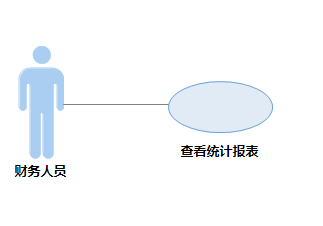
\includegraphics[width=.5\textwidth]{fig/276001.png}
    \caption{用例图:查看统计报表}
    \label{fig:276001}
\end{figure}

\subsubsection{系统顺序图}

\begin{figure}[H]
    \centering
    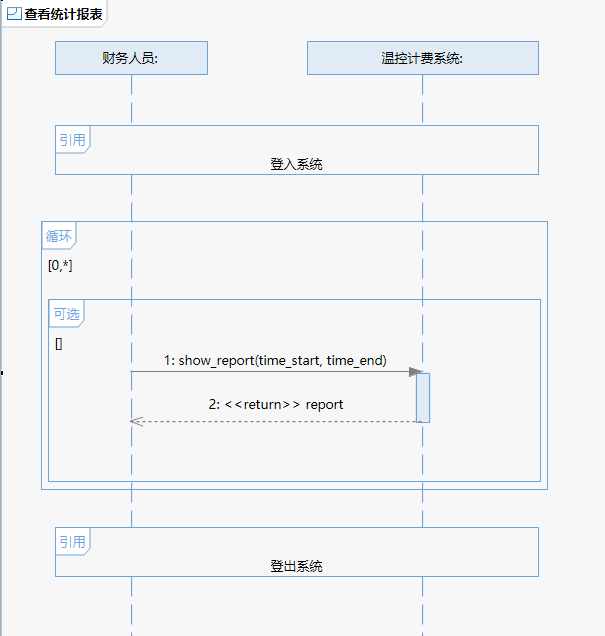
\includegraphics[width=.8\textwidth]{fig/276002.png}
    \caption{系统顺序图:查看统计报表}
    \label{fig:276002}
\end{figure}

\subsubsection{操作契约}

\begin{center}
    \begin{tabular}{|>{\centering}m{0.15\textwidth}|m{0.7\textwidth}|}
        \hline
        系统事件                  & \multicolumn{1}{l|}{\code{show\_report(time\_start, time\_end)}} \\
        \hline
        交叉引用                  & 查看统计报表                                                     \\
        \hline
        前置条件                  & 财务人员登入财务系统,要求查看报表                               \\
        \hline
        \multirow{4}{*}{后置条件} & 一个新的(概念类)统计报表被创建                                 \\
        \cline{2-2}
                                  & 统计报表与财务人员建立关联                                       \\
        \cline{2-2}
                                  & 统计报表与温控计费系统建立关联                                   \\
        \cline{2-2}
                                  & 统计报表的属性初始化:报表编号,开始时间,结束时间,费用等       \\
        \hline
    \end{tabular}
\end{center}

\subsection{生成使用账单}
\subsubsection{用例图}

\begin{figure}[H]
    \centering
    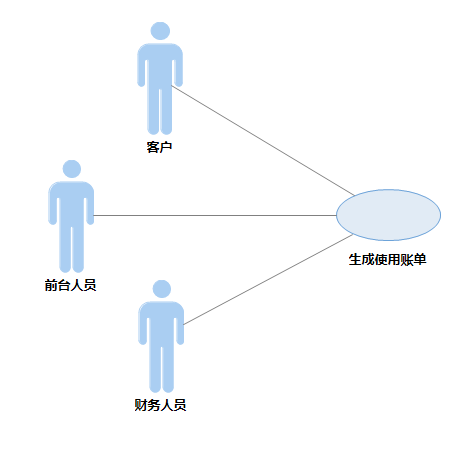
\includegraphics[width=.5\textwidth]{fig/276003.png}
    \caption{用例图:生成使用账单}
    \label{fig:276003}
\end{figure}

\subsubsection{系统顺序图}

\begin{figure}[H]
    \centering
    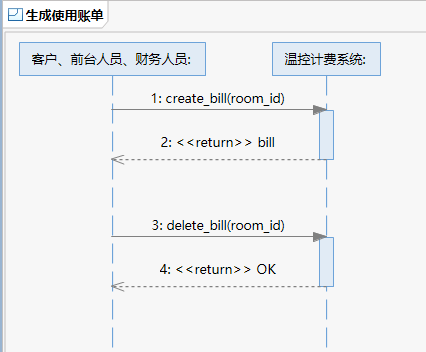
\includegraphics[width=.8\textwidth]{fig/276004.png}
    \caption{系统顺序图:生成使用账单}
    \label{fig:276004}
\end{figure}

\subsubsection{操作契约}

\begin{center}
    \begin{tabular}{|>{\centering}m{0.15\textwidth}|m{0.7\textwidth}|}
        \hline
        系统事件                  & \multicolumn{1}{l|}{\code{create\_bill(room\_id)}}       \\
        \hline
        交叉引用                  & 生成使用账单                                             \\
        \hline
        前置条件                  & 操作者请求查看使用账单                                   \\
        \hline
        \multirow{4}{*}{后置条件} & 一个新的(概念类)使用账单被创建                         \\
        \cline{2-2}
                                  & 使用账单与操作者(客户、前台人员、财务人员)建立关联     \\
        \cline{2-2}
                                  & 使用账单与温控计费系统建立关联                           \\
        \cline{2-2}
                                  & 使用账单的属性初始化:账单编号,房间号,使用时间,费用等 \\
        \hline
    \end{tabular}
\end{center}

\begin{center}
    \begin{tabular}{|>{\centering}m{0.15\textwidth}|m{0.7\textwidth}|}
        \hline
        系统事件                  & \multicolumn{1}{l|}{\code{delete\_bill(room\_id)}}           \\
        \hline
        交叉引用                  & 删除使用账单                                                 \\
        \hline
        前置条件                  & 操作者请求删除使用账单                                       \\
        \hline
        \multirow{3}{*}{后置条件} & 一个(概念类)使用账单被删除                                 \\
        \cline{2-2}
                                  & 使用账单与操作者(客户、前台人员、财务人员)之间的关联被消除 \\
        \cline{2-2}
                                  & 使用账单与温控计费系统之间的关联被消除                       \\
        \hline
    \end{tabular}
\end{center}

\end{document}